\documentclass{article}
\usepackage[final]{nips_2017}
\usepackage[utf8]{inputenc} % allow utf-8 input
\usepackage[T1]{fontenc}    % use 8-bit T1 fonts
\usepackage{hyperref}       % hyperlinks
\usepackage{url}            % simple URL typesetting
\usepackage{booktabs}       % professional-quality tables
\usepackage{amsfonts}       % blackboard math symbols
\usepackage{nicefrac}       % compact symbols for 1/2, etc.
\usepackage{microtype}      % microtypography
\usepackage{graphicx}
\usepackage{todonotes}
\let\svtodo\todo\renewcommand\todo[1]{\svtodo[inline]{#1}}
\title{\Large Deep Reinforcement Learning for Unsteady Flow Control}
\usepackage{siunitx}
\usepackage{wrapfig}
\usepackage{amsmath}
\usepackage{cleveref}
\usepackage{subfig}

\author{
  Anthony Corso \\
  Department of Aeronautics and Astronautics\\
  Stanford University\\
  \texttt{acorso@stanford.edu} \\
}

\begin{document}
% \nipsfinalcopy is no longer used

\begin{center}

\includegraphics[width=3cm, height=0.7cm]{CS230}
\end{center}

\maketitle

\begin{abstract}
Unsteady flow control remains a difficult task for even the most advanced control techniques, and if solved, could benefit many industrial applications. This work demonstrates that deep reinforcement learning can be used to discover control policies for active flow control. Vortex shedding behind a 2D circular cylinder is studied and a functional control policy is learned for a Reynolds number of 50. Multiple reinforcement learning algorithms and architectures are compared and contrasted. Additional analysis reveals that the near-wake flow-field is most important when designing a control policy. 
\end{abstract}

\section{Introduction}	
Unsteady flow control remains a difficult task for even the most advanced control techniques. Control in this domain is challenging because the dynamics of an unsteady fluid system are nonlinear, high-dimensional, and continuous. Solving the flow-control problem, however, could have a big payoff for many industrial applications including energy generation, transportation, climate control, and chemical processing.

This work focuses on a canonical flow-control problem: the suppression of vortices behind a cylinder in a 2D flow field (see \cref{fig:suppresion} for an example). The appearance of vortex shedding is governed by a flow parameter called the Reynold's number, given by $ \mathcal{R} = \frac{\rho U_\infty D}{\mu}$ where $U_\infty$ is the freestream velocity, $\rho$ is the fluid density, $\mu$ is the fluid viscosity, and $D$ is the diameter of the cylinder. When the Reynold's number is larger than a critical threshold (in this case $\mathcal{R} > 45$), then small perturbations in a steady flow field can grow into oscillating vortices that a shed into the wake of the cylinder. Vortex shedding leads to increased drag on the cylinder, and is generally undesirable when considering the performance of aerodynamic systems. These vortices can be disrupted and suppressed by injecting momentum and energy into the flow field in a highly specific manner. The two most common ways of suppressing vortices are by rotating the cylinder to use frictional forces to add energy to the flow (the focus of this work), or by using jets to inject momentum and energy directly (the focus of related work).

The best control policy for when and how to inject momentum into the fluid is difficult to discern. This work attempts to cast the problem of unsteady flow control as a Markov Decision Procress (MDP) and apply deep reinforcement learning (RL) techniques to automatically find a viable control policy. Deep reinforcement learning uses a Deep Neural Network (DNN) to encode a mapping from system state to control action, and optimize that mapping to achieve good performance on a desired task. For the problem of flow control, the state (or input to the reinforcement learning algorithm) is a snapshot of the flow-field around the circular cylinder. In this case, the snapshot contains density, $x$-velocity, $y$-velocity, and energy values on a $256 \times 128$ grid. The output of the DRL control policy will be the angular velocity of the cylinder. If the action space is continuous then this will correspond to a single real value, but if it is discrete then the angular velocity will be binned into a user-specified range of values.

This paper is organized as follows: \cref{sec:related} gives a brief overview of past work to give context to this problem. Then \verb|gym-pyfr| is presented in \cref{sec:data} as a new framework for solving flow control problems using RL methods. The methods applied to the vortex suppression problem are discussed in \cref{sec:methods} and the results of several experiments are given in \cref{sec:experiments}. Lastly, \cref{sec:conclusion} concludes and gives directions for future work.


\section{Related work}
\label{sec:related}
Traditionally the problem of vortex suppression behind a circular cylinder has been studied experimentally \cite{bearman2004experimental} or in a traditional control framework \cite{homescu2002suppression}. Experimentation is costly and can be unprincipled, while the use of traditional control techniques can be challenging for a system as complicated as the unsteady Navier-Stokes equations. \cite{homescu2002suppression} used optimal control strategies to solve for the optimal control policy for vortex suppression, but need to solve a complicated set of equations to do so, making it difficult to extend this methodology to other types (and more complicated) problems.

There has recently been some work applying Deep Neural Networks (DNNs) to solve the vortex suppression problem. \cite{morton2018deep} used a DNN to learn a linearization of the dynamics of the system and then applied model predictive control to suppress the vortex shedding (using cylinder rotations) at a Reynolds number of 50. This work also demonstrated that flow control (at $\mathcal{R} = 50$) can be achieved using a proportional controller based on the $y$-velocity of the fluid at a specific point in the wake ($0.4$ times the diameter of the cylinder). The appropriate gain was found to $0.88$.  \cite{rabault2018deep, rabault2019artificial} used the proximal policy optimization algorithm to learn a control policy for sucking and blowing jets on the surface of a cylinder. traditional PPO was insufficient to solve the control problem, however, and the authors used several tricks to get the policy to be continuous and smooth which sped up the learning process. Positive results were achieved for a Reynolds number of $\mathcal{R} = 100$. The reward function that was used in this case was a function of drag and lift on the cylinder.

\section{RL Framework for Flow Control (Data)}
\label{sec:data}

There are several limitations of many modern fluid flow simulations that make them difficult to use with existing reinforcement learning frameworks. First, they are often setup via a configuration file or other non-programmatic setup (like a GUI), making it difficult to dynamically generate many simulations. Second, fluid simulations are notoriously slow due to the difficulty of accurately solving the Navier-Stokes equations. Lastly, simulators often have interfaces that do not allow for interaction with the simulation while it is running.  To address these limitations and to help bring RL to the fluids community, this work presents \verb|gym-pyfr| a new, open-source, framework for solving flow control problems with RL. The framework is built on top of two outstanding modules, \verb|OpenAI gym| \cite{brockman2016openai} and \verb|PyFR| \cite{witherden2014pyfr}. 

\verb|PyFR| is an open-source flow simulation package written in python that achieves good simulation performance using GPU computing. To accelerate the performance for the cylinder problem for this work, the cylinder mesh was made as coarse as possible (through trial and error) while still retaining solution accuracy. The original mesh used for rotational flow control had 3234 elements while the newly created mesh has only 653 and runs about $10\times$ faster.

\verb|OpenAI gym| is a python module that provides a common interface for solving RL problems. To bring \verb|PyFR| into a gym environment, a lot of work had to be done to modularize the running of \verb|PyFR| and allow simulations to be setup programmatically. A gym environment must provide three main functions to be used with most existing reinforcement learning algorithms: \verb|init|, \verb|step|, and \verb|reset|. Below is a description of what each of these functions do in the context of a \verb|gym-pyfr| environment.

\begin{itemize}
    \item \verb|init(options)| - Initializes the observation space to be $256 \times 128 \times 4$ ($128 \times 256$ grid with 4 degrees of freedom at each point) and the actions space to be either continuous and 1D (the rotational velocity of the cylinder) or discretized into a desired number of bins. A \verb|PyFR| object (see appendix for details) is created based on the user-specified options such as the desired $\mathcal{R}$ and episode length parameters.
    \item \verb|step|$(a)$ - This function first sets the cylinder rotation based on the specified action, $a$. Then the simulation is advanced by one timestep and the reward at the new state is observed. Lastly, the timestep is checked to see if the end of the episode has been reached. The function returns the new observation, the reward, and a flag indicating episode completion.
    \item \verb|reset|() - This function re-initializes the \verb|PyFR| object back to its starting state and returns the state of flow field.
\end{itemize}


\section{ Methods }
\label{sec:methods}
This sections outlines the formulation of the problem statement in more detail and describes the specific algorithms and architectures that are used for its decision. 

\subsection{Markov Decision Process Formulation}
In order for this problem to be solved using common DRL algorithms, we formulate it as a Markov Decision process which is a 5-tuple of the form ($\mathcal{S}$, $A$, $P$, $\gamma$, $R$). $\mathcal{S}$ is the state space, $A$ is the action space, $P$ is a the transition probability, $\gamma$ is the discount factor, and $R$ is the reward function (which is detailed in the following subsection). For this problem, the following are defined as
\begin{itemize}
\item $\mathcal{S}$ is a (128,256,4) tensor that stores the flow-field information at each gridpoint
\item $\mathcal{A}$ is a continuous variable $\omega$ that represents the angular velocity of the cylinder
\item $\mathcal{P}(\mathcal{S}' \mid \mathcal{S}, a)$ is a deterministic function governed by the Navier-Stokes equations
\item The discount factor will be set to $\gamma = 0.9$ so the algorithm attempts to suppress the shedding as quickly as possible.
\end{itemize}

The goal of a reinforcement learning algorithm is to learn a mapping $p(a) = \pi^*(s)$ (the optimal policy) that determines a probability distribution for the best action to take given the current state $s$. Some RL algorithms seek to learn $\pi^*$ directly while others try to learn another function known as the optimal state-action value function $Q^*(s,a)$ which returns the expected sum of future rewards when following an optimal policy. The optimal policy can then be extracted from this function from 

\[ \pi^*(s) = \max_{a} Q^*(s,a) \]

\subsection{Reward Function}


% \begin{wrapfigure}{r}{0.4\textwidth}
%   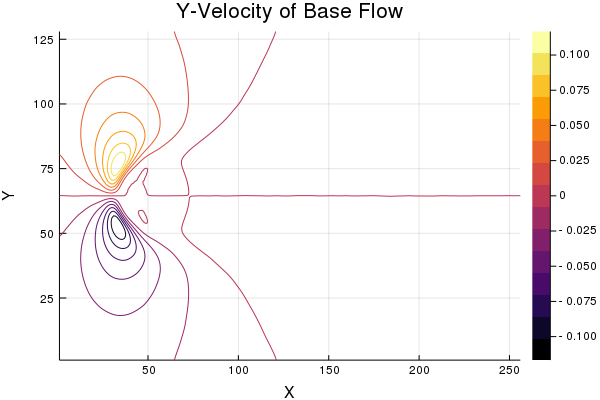
\includegraphics[width=0.4\textwidth]{base_flow}
%   \caption{Target flow field }
%   \label{fig:base_flow}
% \end{wrapfigure}

A reward function must be selected so that it guides an RL algorithm to produce a flow field that is steady in the wake of the cylinder. In this work, we take the approach of finding a baseline flow-field that is steady, and then giving a reward based on how close the current flow-field is to the baseline. To make this more concrete, we can define the reward $r$ to be 
\begin{equation}
    r(s,a) = -\left\lVert x - x_b \right\rVert_2
\end{equation}
where $x$ is a vector containing each degree of freedom for each point in the flow field, and $x_b$ is the baseline flow state.

The baseline flow fields for this work were found by running the fluid simulation with vortex shedding and then tim-averaging the solution to get a pseudo-steday flow solution. Although this approach does not give the true steady-state profile, it is close enough to encourage vortex suppression.

\subsection{Algorithms and Network architecture}

Two Deep RL algorithms were used and compared, Deep Q-Learning (DQN) \cite{mnih2013playing} and Proximal Policy Optimization (PPO) \cite{schulman2017proximal}.  DQN is a value-function approximation method which means that it uses a DNN to approximate the optimal state-action value function $Q^*$. It uses an experience replay buffer to store and reuse previous data points to improve sample efficiency. PPO is a policy gradient method which means that is uses a DNN to approximate the mapping $\pi^*(s)$ directly. Implementations of these two algorithms were used from the python module \verb|stable-baselines| \cite{stable-baselines}.


Two different networks will be referenced in the experimentation section. The first is a basic multi-layer perception (MLP) that has two hidden layers, each with 64 units and a ReLU activation for each layer. The second is a convolutional neural network (CNN) that has the same architecture as \cite{mnih2015human} which involves three convolutional layers (\num{32} $(8 \times 8)$ filters with stride \num{4},  \num{64} $(4 \times 4)$ filters with stride \num{2}, and \num{64} $(3 \times 3)$ filters with stride \num{1}, respectively). Then a fully connected hidden layer with 512 ReLUs. The output layer is fully connected with an output for each action in the action space. 

\section{Experiments}
\label{sec:experiments}

The goal of the experiments was three fold: 1) Compare different network architectures and algorithms to see which is the most promising for continued research, then 2) find a control policy with the most promising approach that could outperform an existing proportional controller (for $\mathcal{R} = 50$), and 3) analyze that controller to gain insight into the problem of vortex shedding. 

To achieve the first goal, we trained two different RL algorithms, tried two different networks, and used two different Reynolds numbers. Experimentation was limited because each training run took between \num{30} - \num{48} hours (7 minutes per episode) to train on a K520 GPU on AWS with the Adam optimization method. The results of training are shown in \cref{fig:learning}. The first comparison was between DQN and PPO both with a CNN network. The DQN algorithm started to learn after about \num{150} episodes and reached high performance after about \num{300}. PPO on the other hand did not learn at all, and actually got stuck simply applying the same action at each timestep. It is unclear why PPO experienced this problem and it is possible that with additional hyperparameter tuning better performance could be achieved. The next comparison was using DQN to compare the MLP network and the CNN network. The MLP also failed to learn any useful polices in the training time allotted. A CNN is a better network choice because convolutional layers are good at quickly localizing important features in a large state-space. Lastly, we took the best architecture (DQN with CNN network) and applied it to the more difficult task of flow control at a higher Reynolds number ($\mathcal{R} = 100$). In this case, the algorithm was not able to achieve a good policy in the training time allotted. Note that the reward is actually much lower for $\mathcal{R} = 100$ shedding due to the larger difference between the steady and unsteady solutions so \num{6600} was added to the reward to bring it to a similar scale as the other experiments.

\begin{figure}
\centering 
    \begin{minipage}{.5\textwidth}
        \centering
        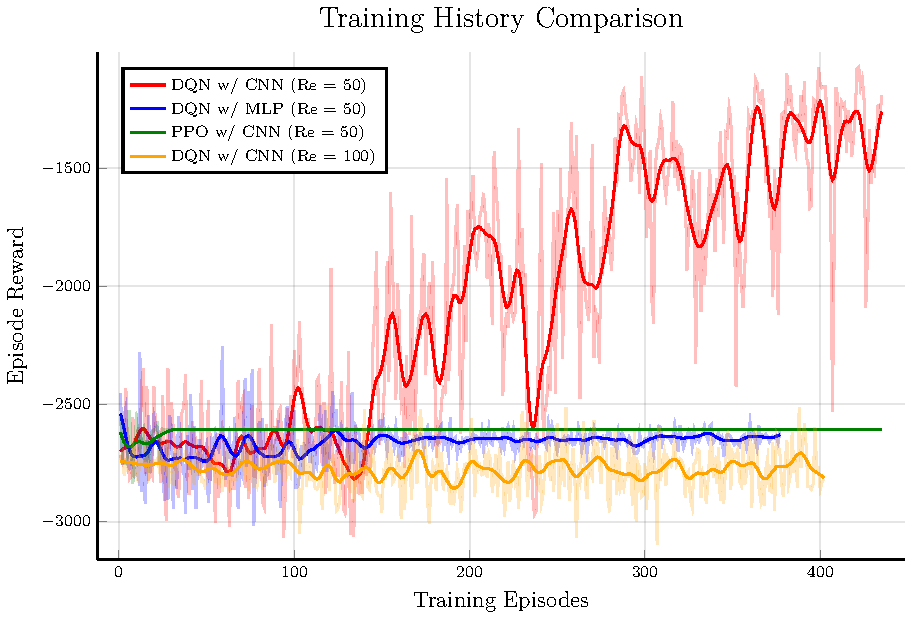
\includegraphics[scale=0.4]{learning}
        \caption{Learning curves of different \\   policy/algorithm combinations}
        \label{fig:learning}
    \end{minipage}%
    \begin{minipage}{.5\textwidth}
        \centering
        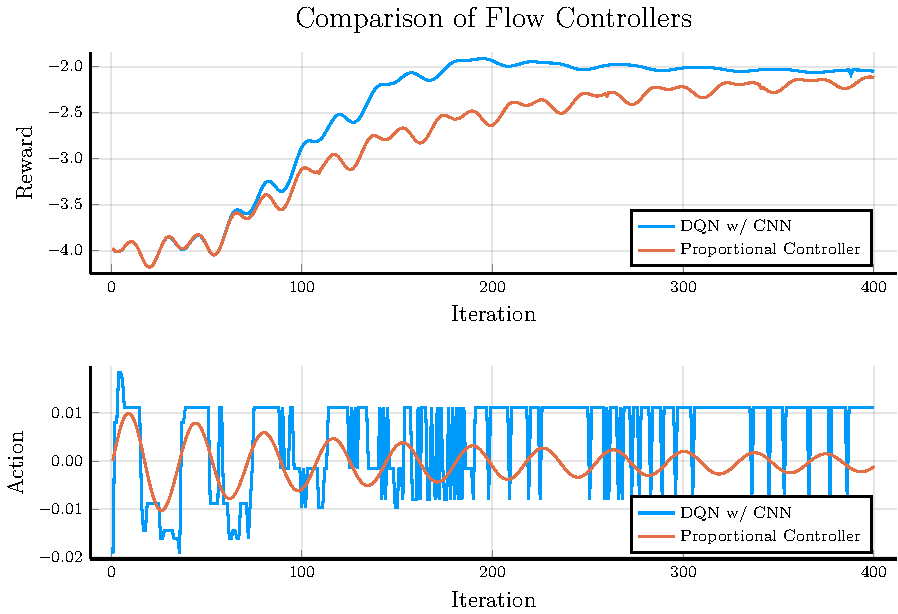
\includegraphics[scale=0.4]{performance}
        \caption{Performance of DQN-trained CNN policy}
        \label{fig:performance}
    \end{minipage}
\end{figure}



Once the best architecture and algorithm was determined, it could be tested on a flow problem and compared to the proportional controller outlined in \cite{morton2018deep}. The results of this comparison are shown in \cref{fig:performance}. In the top graph we can see that the CNN policy was able to suppress the vortex shedding more quickly than the proportional controller, obtaining a larger total reward. In the bottom graph we can compare the control law found by the RL algorithm to the control law of a proportional controller. In the first part of episode (up to iteration ~125), both control laws look somewhat similar, especially when you compare the sign). Once the vortices have mostly been suppressed, then the two algorithms had different control strategies for maintaining the suppression. The RL algorithm spends most of its control effort with a positive rotation while the proportional controller continues to oscillate at low amplitude. Snapshots of the $y$-velocity of the state space are shown in \cref{fig:suppresion} for different iterations during the suppression process.

\begin{figure}
\vskip -0.4in
    \subfloat[Iteration 0]{\label{iter0}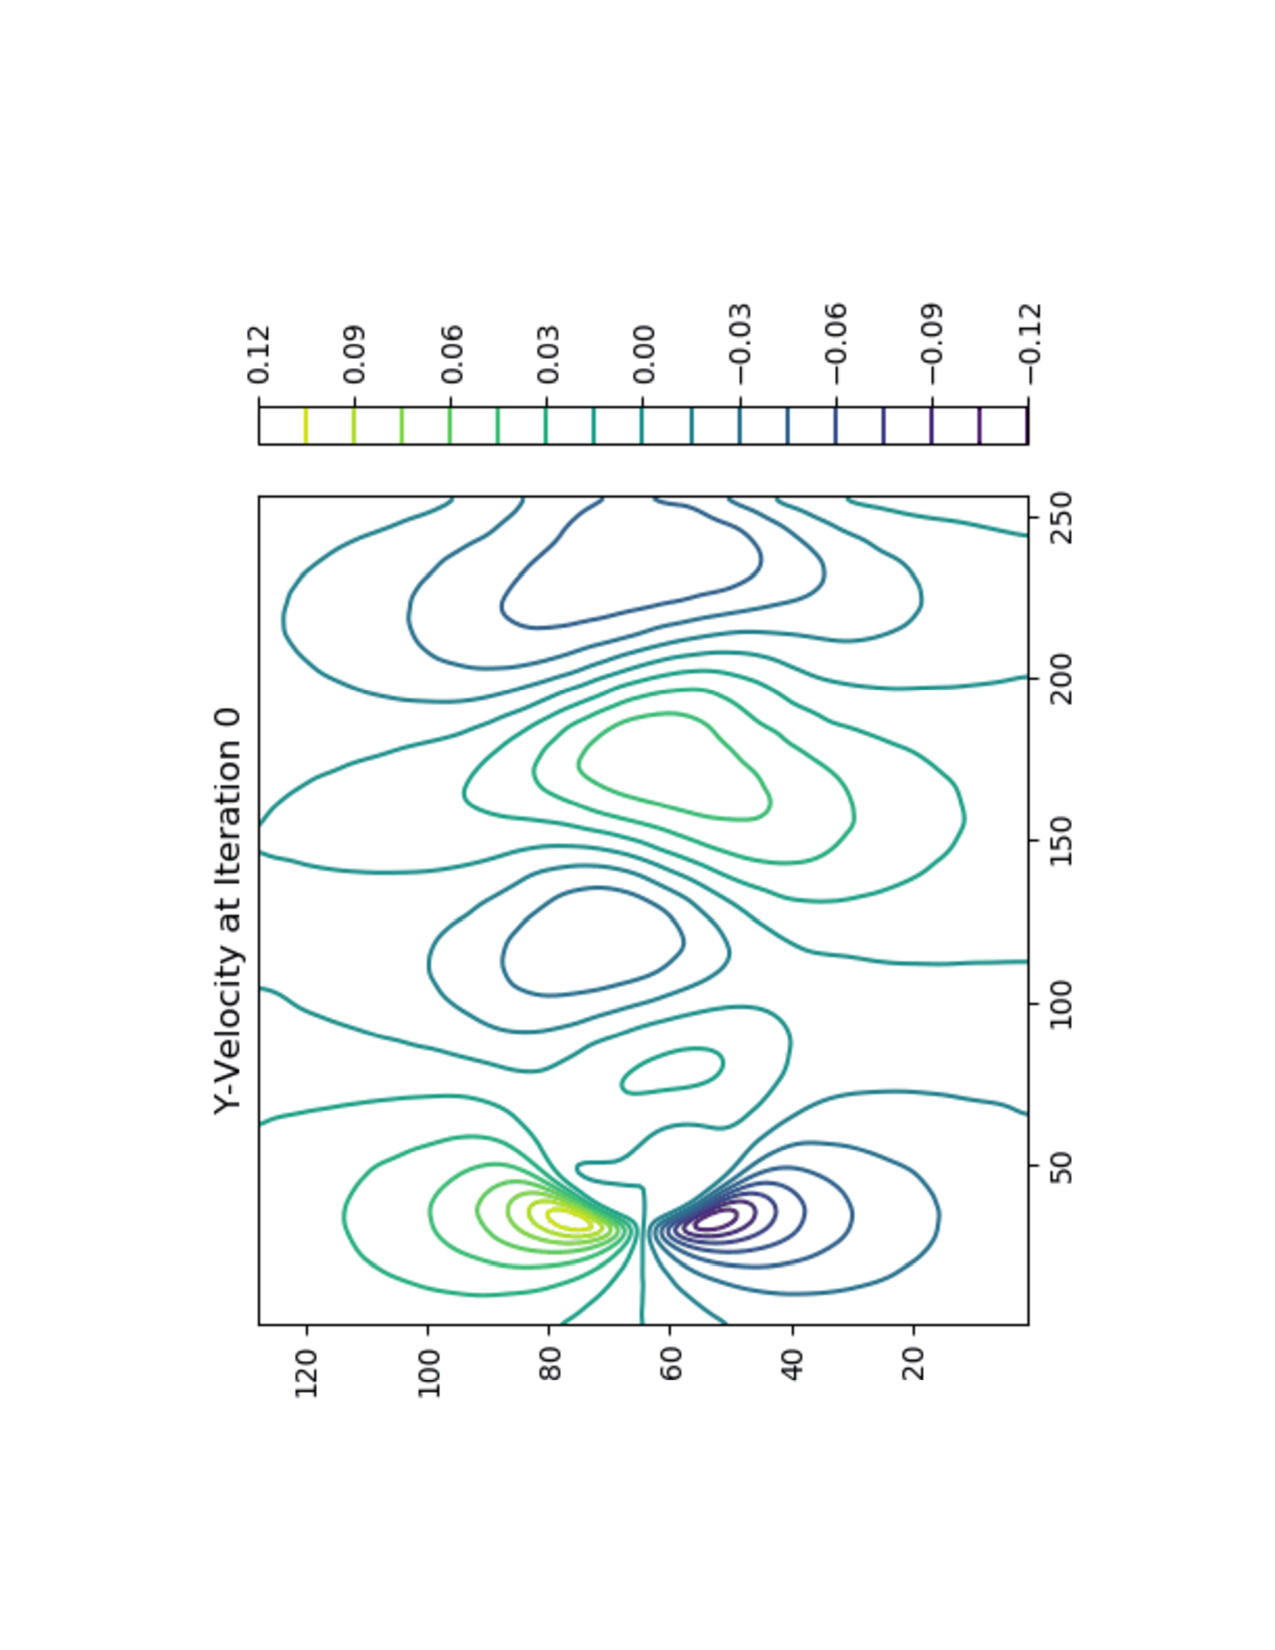
\includegraphics[angle = 270, width=0.4\textwidth]{./s1}}
    \hspace*{-0.4in}
    \subfloat[Iteration 150]{\label{iter150}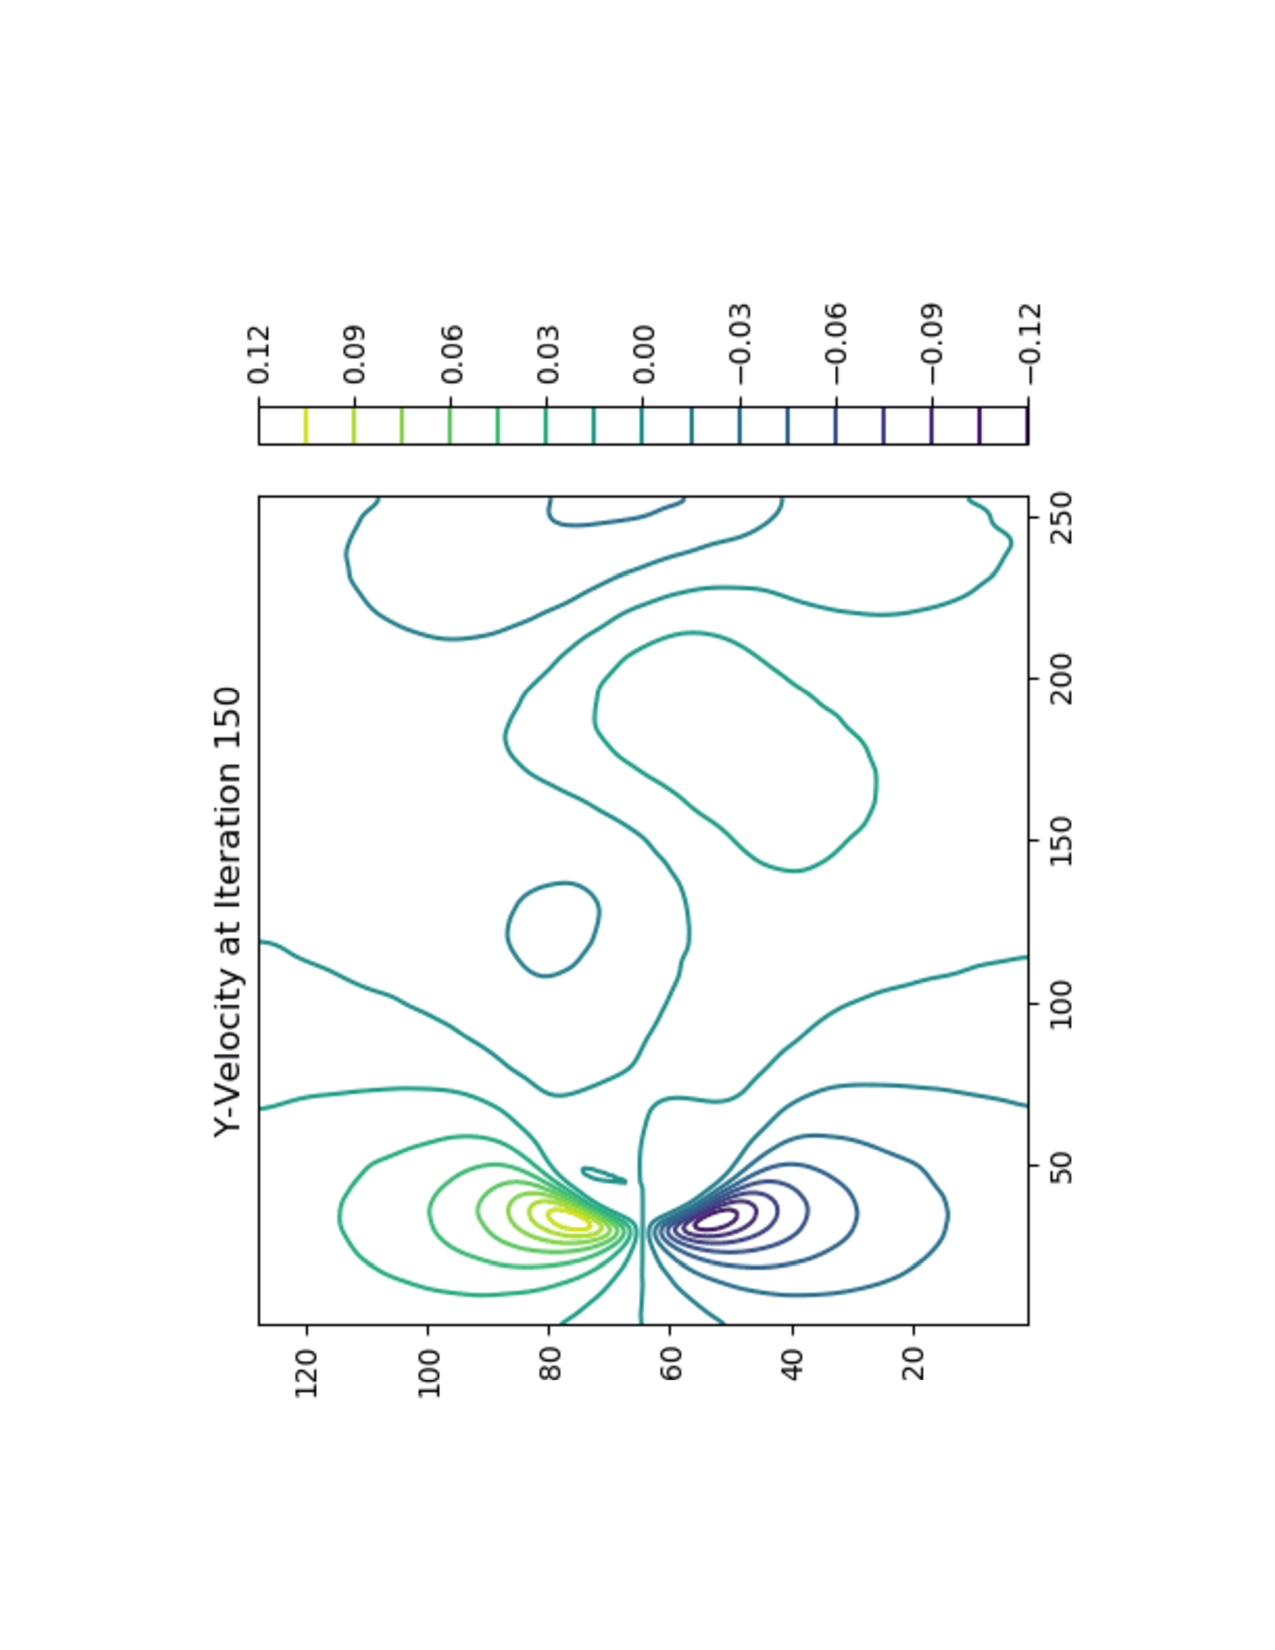
\includegraphics[angle = 270,width=0.4\textwidth]{./s2}}
    \hspace*{-0.4in}
    \subfloat[Iteration 300]{\label{iter300}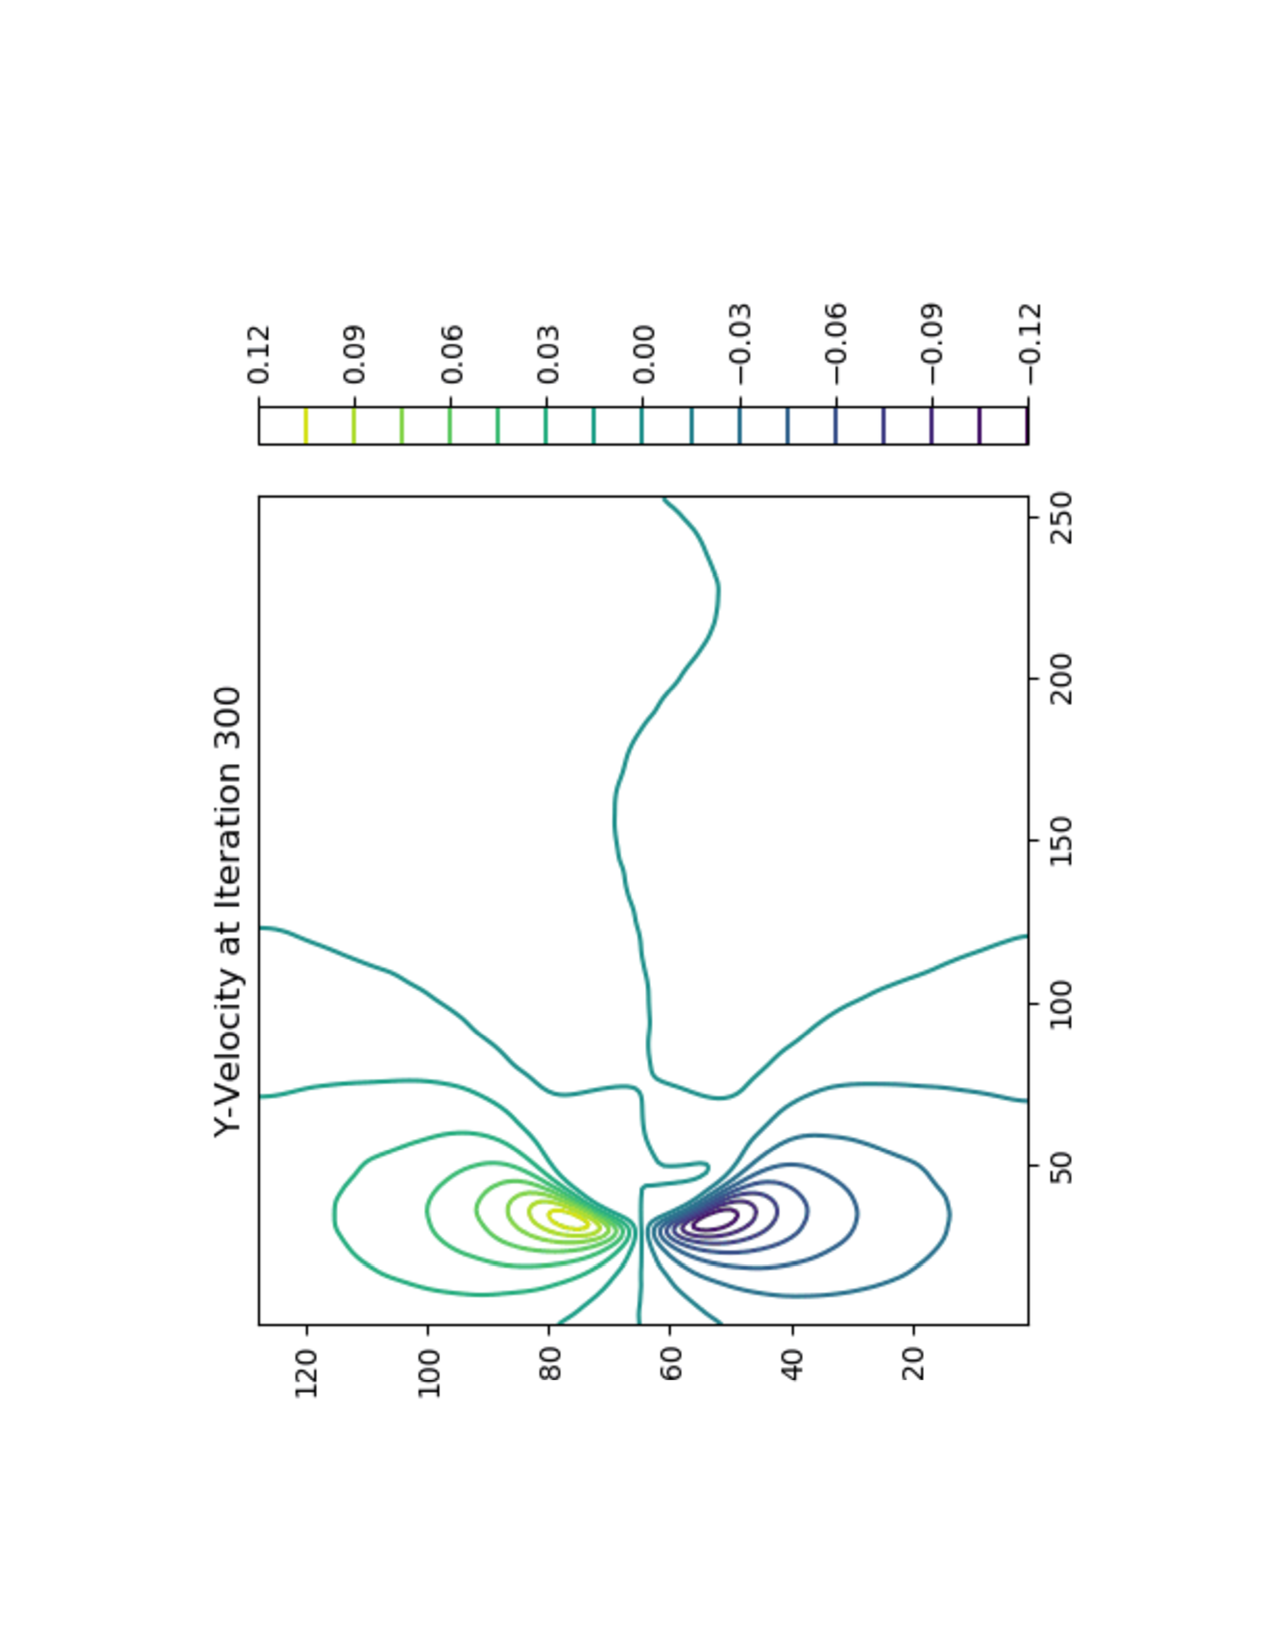
\includegraphics[angle = 270,width=0.4\columnwidth]{./s3}}
    \caption{Vortex shedding suppression at $\mathcal{R} = 50$ using a DQN-trained CNN state-action value function}
    \label{fig:suppresion}
    \vskip -0.2in
\end{figure}




Lastly, to visualize what the network is looking at when making action decisions, a saliency map was generated using \cite{saliency}. On iterations 0, the state is fed to the network and the gradient was backpropogated from the selected action ($\omega$ = -0.02) to the input. The magnitude of the gradient was then plotted in \cref{fig:saliency} where the red circle shows where the cylinder is located. We can see from the saliency map that the network is primarily focused on the near-wake of the cylinder as the most important region. Regions in front of of the cylinder and outside of the wake are not deemed important at all. Additionally we can observe an asymmetry in the saliency for this action which is to be expected for an asymmetric action (i.e. to choose a negative rotation velocity, the network is more concerned with the flow pattern in the upper region of the wake). 
\begin{wrapfigure}{r}{0.5\textwidth}
\centering
  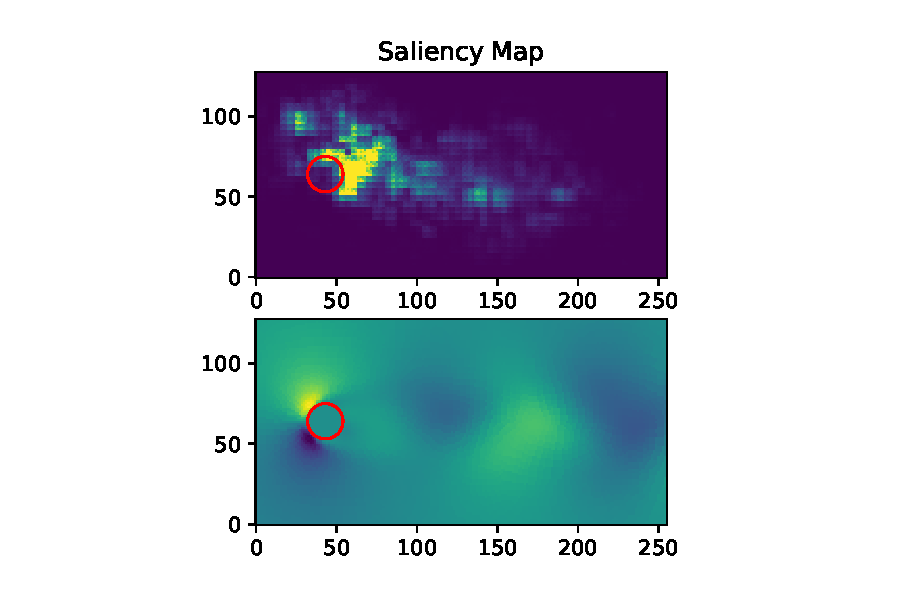
\includegraphics[scale=0.7]{saliency_map}
  \caption{Saliency map for taken action on first iteration}
  \label{fig:saliency}
\end{wrapfigure}

\section{Conclusion and Future Work}
\label{sec:conclusion}

The results of these experiments demonstrate that it is feasible to using deep reinforcement learning to discover a control policy for vortex suppression behind a circular cylinder via rotation. The best algorithm seems to be a DQN coupled with a CNN value network but further experimentation should be conducted. The methods has only been shown at lower Reynolds number and will likely require modifications or longer training times for larger Reynolds numbers. 

Future work on this topic could include
\begin{itemize}
    \item Using transfer learning from a linearization network \cite{morton2018deep} to accelerate the feature extraction process of the learning. 
    \item Replace the compressible flow solver with an incompressible solver that can run much more quickly
    \item Implement the capabilities of sucking and blowing jets to compare the efficacy of the approaches.
    \item Use a different reward function such as the drag or vorticity of the flow field
\end{itemize}

% \pagebreak
% \section{Contributions}
% I worked as a group of one on this project and was therefore responsible for completing all tasks on this project. I would like to acknowledge, however, the input from Dr. Freddie Witherden and Jeremy Morton for their assistance in making PyFR compatible for this flow-control problem. 

\bibliography{cs230}
\bibliographystyle{cs230}

% \appendix
% \section{DQN and PPO Description}
% \label{sec:alg}

% \subsubsection{Deep Q-Learning}
% Deep Q-Learning \cite{mnih2013playing} is DRL algorithm that seeks to estimate that state-action value function $Q(s,a)$ using a DNN. If we knew the true optimal state-action value function $Q^*(s,a)$ then we could train a neural network approximation to that function,  $\hat{Q}(s,a \mid \theta)$, parameterized by weights $\theta$, using a least-squares loss function defined by 

% \begin{equation}
%     L(\theta) = \mathbb{E}_{s \in \mathcal{S}, \ a \in \mathcal{A}}\left[ \left( Q^*(s,a) - \hat{Q}(s,a \mid \theta) \right)^2 \right]
% \end{equation}
% The problem, however, is that $Q^*$ is not known. To estimate it, we use another neural network called the \textit{target network} which is parameterized by a different set of weights $\phi$ such that 
% \begin{equation} Q^*(s,a) \approx \mathbb{E}_{s' \in \mathcal{S}}\left[ r + \gamma \max_{a' \in \mathcal{A}} \hat{Q}(s',a' \mid \phi) \right]
% \end{equation}
% In a procedure called bootstrapping, $\phi_i = \theta_{i-1}$ (i.e. the target weights are set to the previous version of the value function weights) which prompts the algorithm to incrementally improve itself. To train a the network $\hat{Q}$ we need the gradient for the loss function with respect to the parameters. For the least-squares loss, the gradient is given by 

% \begin{equation}
%     \nabla_\theta L(\theta) = \mathbb{E}_{s, s' \in \mathcal{S}, \ a \in \mathcal{A}}\left[ \left( r + \gamma \max_{a' \in \mathcal{A}} \hat{Q}(s',a' \mid \phi) - \hat{Q}(s,a \mid \theta) \right) \nabla_\theta \hat{Q}(s,a \mid \theta)  \right]
% \end{equation}
% The gradient of the network $\nabla_\theta \hat{Q}(s,a \mid \theta)$ can be computed using conventional backpropagation procedures. In practice, it is not feasible to take an expectation over states so instead we employ a stochastic gradient descent technique and apply the gradient for each observed transition $(s, a, s')$.

% There were two additional tricks that are often used to improve the stability and performance of the DQN algorithm that were also employed in this work. First, the target network weights $\phi$ are fixed for a specified number of iterations (500 in this work) before they are updated to the value network weights again. This improves the stability of the training procedure. Second, an buffer of old state-action-state pairs are stored in \textit{experience replay buffer} and sampled randomly for training at each timestep. This breaks the temporal correlation of samples can improves learning performance. Given the size of the state space, in this work we were limited to a replay buffer of \num{5000} observations but buffers of \num{50000} are more common. 

% The algorithm runs as follows. At each timestep in the simulation, an action is selected by either choosing the action with the largest $Q$ value or selecting an action at random. The simulation is stepped forward with that action and the result is stored in the replay buffer. The replay buffer is then sampled from and used to update the weights of the value network. The simulation resets at the end of each episode but the weights are retained. The process continues until a fixed number of iterations has passed or the policy has reached a desired level of effectiveness.

% \subsubsection{Proximal Policy Optimization}
% In contrast to DQN, Proximal Policy Optimization (PPO) \cite{schulman2017proximal} is a policy-gradient method which seeks to use a DNN to directly approximate the optimal control policy using a network parameterized by the weights $\theta$ given by  $\hat{\pi}^*_\theta(a \mid s)$ where $a \mid s$ represents a probability distribution over actions. The loss function for PPO is 

% \begin{equation}
%     \label{eqn:ppo}
%     L^{\rm PPO}(\theta) = \mathbb{E}_{\pi_\theta}\left[ \min(r_t(\theta) \hat{A}_t, \ {\rm clip}(r_t(\theta), \ 1-\epsilon, \ 1 + \epsilon) 
%     \hat{A}_t \right]
% \end{equation}

% where the likelihood ration $r_t$ is given by 
% \begin{equation}
%     r_t(\theta) = \frac{\pi_\theta(a_t \mid s_t)}{\pi_{\theta_{\rm old}}(a_t \mid s_t)}
% \end{equation}
% and $\hat{A}_t$ is an estimator for the advantage function $A(s,a) = Q(s,a) - \bar{Q}(s,a)$ where the bar denotes averaging over actions. For this work $A$ was estimated using a generalized advantage estimator [Citation]. The expectation in \cref{eqn:ppo} is over state-action-state observations seen under the policy $\pi_\theta$. The clip function limits the gradients of the policy and creates a pessimistic bound on the true objective function which improves training stability.

% PPO runs for a fixed number of iterations, letting the current policy gather trajectories in the simulation. These trajectories are used to compute the advantage function at each timestep and the total loss from all of the trajectories. The gradient of the loss is then used to update the policy parameters to improve the policy. The process continues until the max number of iterations is reached or the policy is considered effective enough.


% \section{PyFR Gym Environment}
% \label{app:gym-pyfr}
% This Appendix details some of the most important user options that have been implemented for the \verb|gym-pyfr| environment and explains their implementation and usage. It also highlights the resources that have been provided in addition to the code (including meshes, initialization files, and baselines). The options are referenced by keyword argument of the \verb|__init__| function of the environment. 

% \begin{itemize}
%     \item \verb|mesh_file| - The location of the mesh used by PyFR. There is no default parameter, the user must specify a mesh. There are two meshes that come with \verb|gym-pyf|: a coarse and fine mesh for the 2D cylinder flow configuration. The coarse mesh runs about $10\times$ faster than the fine mesh.
%     \item \verb|init_file| - The initial solution file (\verb|*.pyfrs|) that PyFR uses to initialize the flow state. \verb|None| is the default and this means that the flow will be initialized to the free-stream parameters set in the config file. \verb|gym-pyfr| provides vortex shedding initialization states for $\mathcal{R} = 50, \ 75, \ 100, \ 125, \ 150, \ 200$. Vortex shedding is initialized by starting with quiescent flow at the desired Reynold's and waiting for small perturbations in the solution to grow to full vortex shedding. For $\mathcal{R} < 100$ the initialization was created by initiating vortex shedding at $\mathcal{R} = 100$ and then reducing the Reynolds number to the desired level. This is a numerical trick that provides the most physically-realistic flow solutions. The other  
%     \item \verb|config_file|  The desired PyFR configuration file. By default the configuration file that is shipped with \verb|gym-pyfr| is used which has all of the desired settings for the 2D cylinder problem. In general it should not be necessary to provide you own configuration file unless you are using features of \verb|PyFR| that \verb|gym-pyfr| does not yet have a programtic interface to. 
%     \item \verb|baseline_file| -  The baseline solution file to compute the reward from. In general this is difficult to come by because having it exactly means solving the problem of unsteady flow at the desired Reynold's number. As a substitute for exact solutions, \verb|gym-pyfr| provides baseline files that come from time-averaging the unsteady vortex shedding solutions to create a quasi-steady baseline to train against. Baselines are provided for $\mathcal{R} = 50, \ 75, \ 100, \ 125, \ 150, \ 200$.
%     \item \verb|discrete| -  Whether or not to discretize the action space. By default this is false and the action space will be continuous and 1D.
%     \item \verb|n| - The number of actions to discretize the action space into if \verb|discrete = True|. The default is 20 but using numbers as high has 50 has been shown to work well with this problem. 
%     \item \verb|action_multiplier| -  Multiplier on the action range. The un-scaled action range is set to be (-2,2) so that initially most actions do not get clipped by OpenAI Gym. The actual actions that are applied in the simulation are the actions that come from the network multiplied by the \verb|action_multiplier| so that the actual default range is (-0.02, 0.02).
%     \item \verb|Re| - This value will set the Reynolds number of the flow by overriding the viscosity of the fluid to 
%     \[ \mu = \mathcal{R}/\sqrt{\gamma} M \]
%     where $M$ is the mach number. Note that this assumes that the length scale of interest is $L=1$ and that the free stream velocity is set to $U_\infty = \sqrt{\gamma} M$. By default this is \verb|None| in which case the Reynold's number of the flow will be set by the configuration file. 
%     \item \verb|tend| - This value will set the end time of the episode and overrides the configuration file end time. By default this is \verb|None| in which case the end time of the epsiode will be set by the configuration file.
% \end{itemize}

\end{document}